\subsection{7.3 Reaction Orders}
\vspace*{0.5em}
Consider $A \longrightarrow B$\\
$[A]_t$ = concentration of $A$ at time $t$\\
$[A]_0$ = concentration of $A$ at time $t=0$
\vspace*{0.5em}

\begin{minipage}{0.99\linewidth}
    \begin{minipage}{0.65\linewidth}
        \begin{align*}
            \parbox{1.3cm}{\textbf{1st Order}}\\
            \text{Rate} &= -\frac{d[A]}{d t} = k[A]^1 \\
            ln[A]_t &= -k t + ln[A]_0
            \\[0.5em]
            \parbox{1.3cm}{\textbf{2nd Order}}\\
            [A]_t& = [A]_0 exp(-k t)\\
            \text{Rate} &= -\frac{d[A]}{d t} = k[A]^2 \\
            \frac{1}{[A]_t} &= k t + \frac{1}{[A]_0}
            \\[0.5em]
            \parbox{1.3cm}{\textbf{Zero Order}}\\
            \text{Rate} &= -\frac{d[A]}{d t} = k[A]^0 = k \\
            [A]_t &= -k t + [A]_0 \\
        \end{align*}
    \end{minipage}
    \begin{minipage}{0.34\linewidth}
        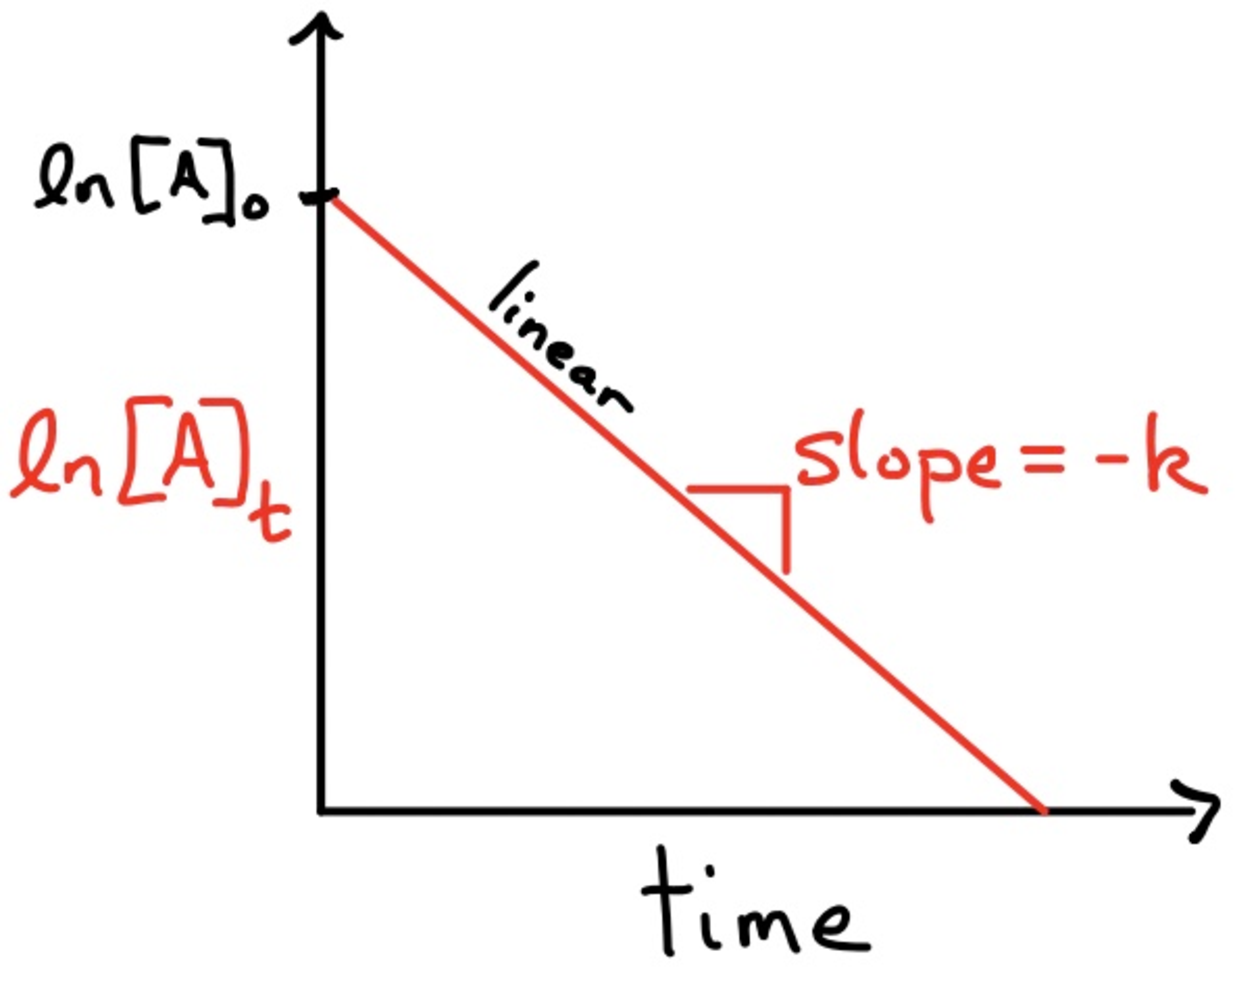
\includegraphics[width=0.9\linewidth]{src/7_Kinetics/images/1st_order.pdf}

        \vspace{1em}
        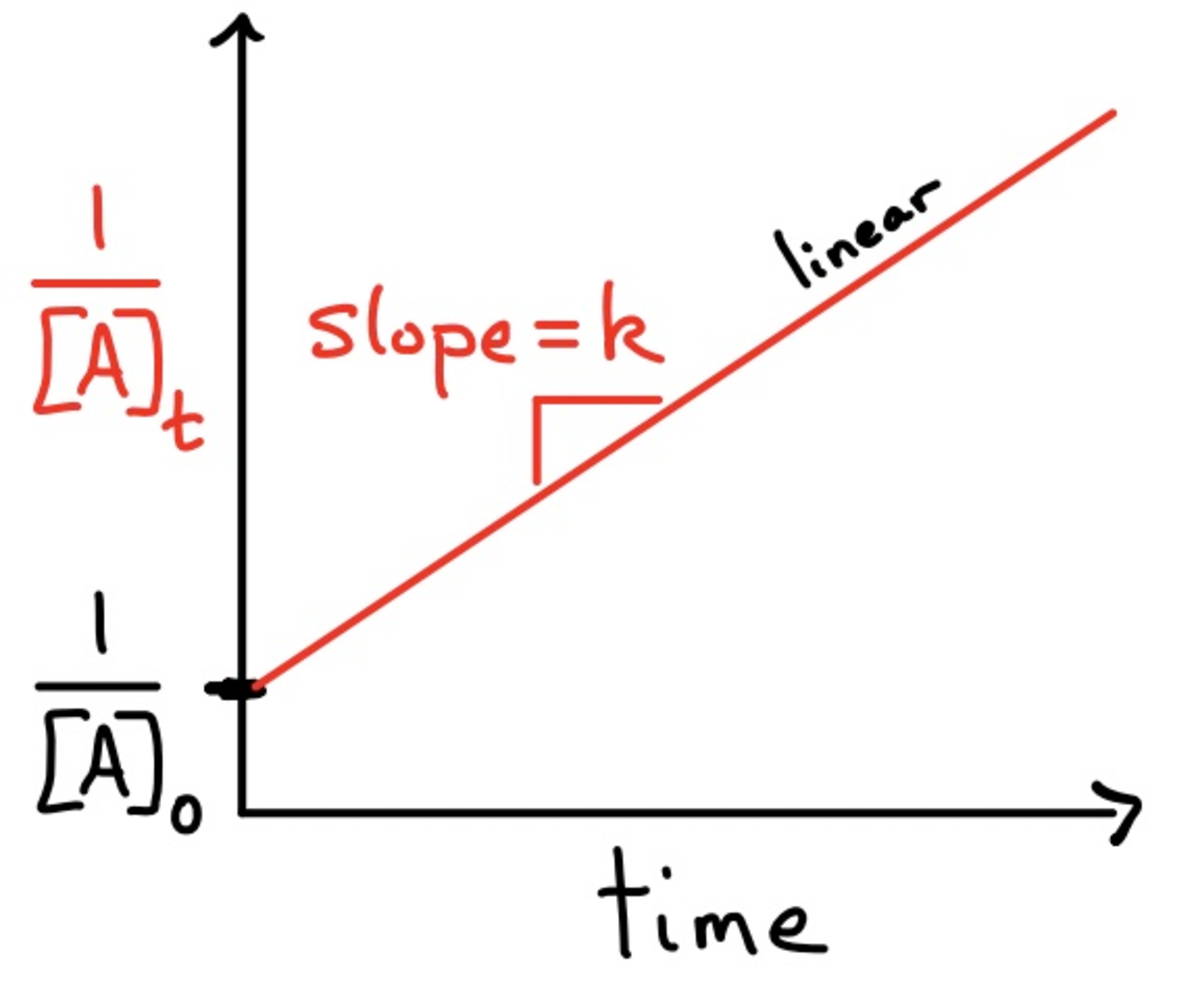
\includegraphics[width=0.9\linewidth]{src/7_Kinetics/images/2nd_order.pdf}

        \vspace{1em}
        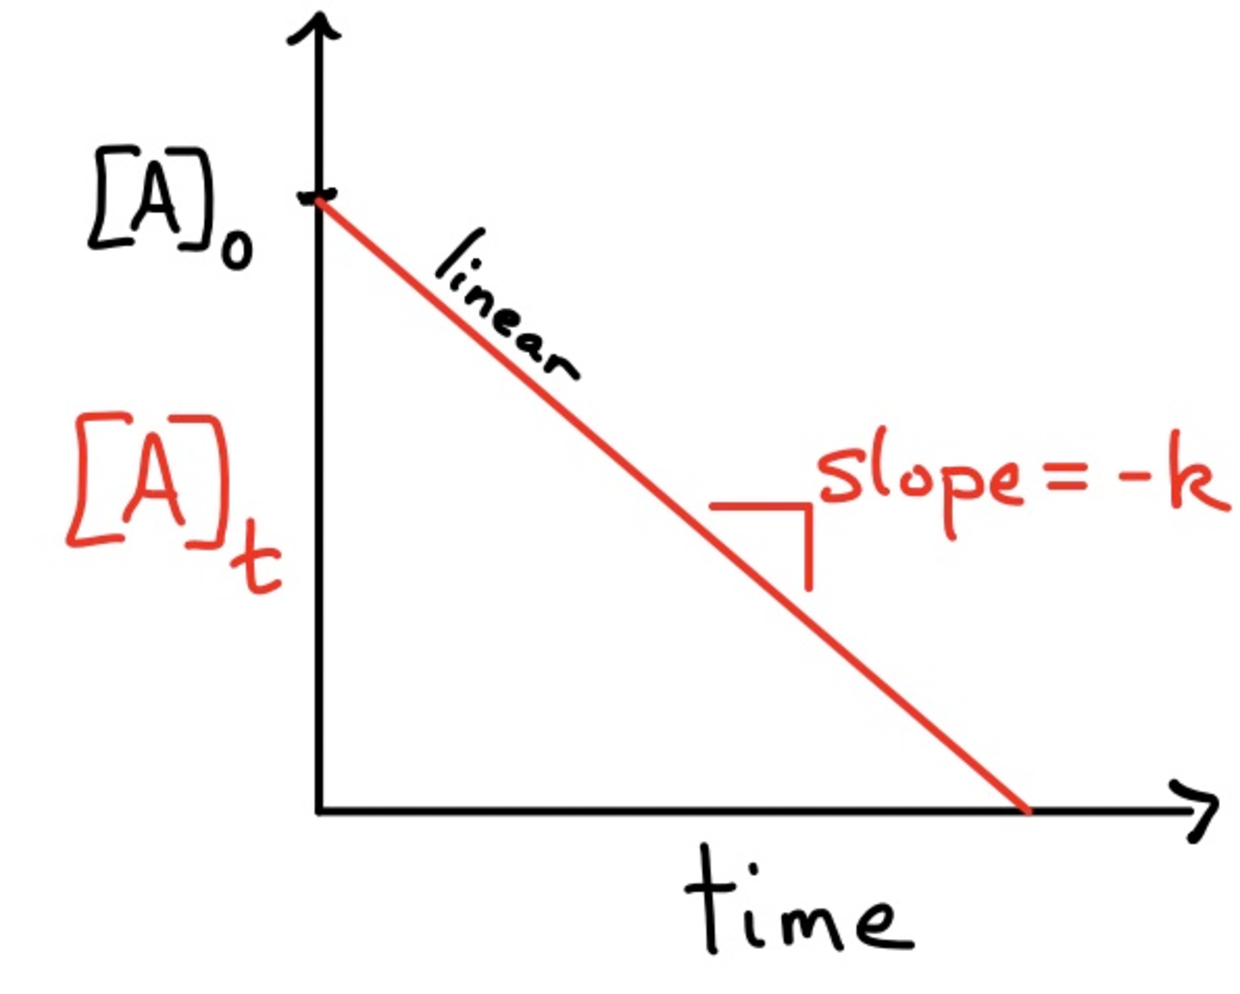
\includegraphics[width=0.9\linewidth]{src/7_Kinetics/images/zero_order.pdf}
    \end{minipage}
\end{minipage}